% Options for packages loaded elsewhere
\PassOptionsToPackage{unicode}{hyperref}
\PassOptionsToPackage{hyphens}{url}
%
\documentclass[
  11pt,
  a4paper,
  onecolumn]{article}
\usepackage{amsmath,amssymb}
\usepackage{iftex}
\ifPDFTeX
  \usepackage[T1]{fontenc}
  \usepackage[utf8]{inputenc}
  \usepackage{textcomp} % provide euro and other symbols
\else % if luatex or xetex
  \usepackage{unicode-math} % this also loads fontspec
  \defaultfontfeatures{Scale=MatchLowercase}
  \defaultfontfeatures[\rmfamily]{Ligatures=TeX,Scale=1}
\fi
\usepackage{lmodern}
\ifPDFTeX\else
  % xetex/luatex font selection
\fi
% Use upquote if available, for straight quotes in verbatim environments
\IfFileExists{upquote.sty}{\usepackage{upquote}}{}
\IfFileExists{microtype.sty}{% use microtype if available
  \usepackage[]{microtype}
  \UseMicrotypeSet[protrusion]{basicmath} % disable protrusion for tt fonts
}{}
\makeatletter
\@ifundefined{KOMAClassName}{% if non-KOMA class
  \IfFileExists{parskip.sty}{%
    \usepackage{parskip}
  }{% else
    \setlength{\parindent}{0pt}
    \setlength{\parskip}{6pt plus 2pt minus 1pt}}
}{% if KOMA class
  \KOMAoptions{parskip=half}}
\makeatother
\usepackage{xcolor}
\usepackage{graphicx}
\makeatletter
\def\maxwidth{\ifdim\Gin@nat@width>\linewidth\linewidth\else\Gin@nat@width\fi}
\def\maxheight{\ifdim\Gin@nat@height>\textheight\textheight\else\Gin@nat@height\fi}
\makeatother
% Scale images if necessary, so that they will not overflow the page
% margins by default, and it is still possible to overwrite the defaults
% using explicit options in \includegraphics[width, height, ...]{}
\setkeys{Gin}{width=\maxwidth,height=\maxheight,keepaspectratio}
% Set default figure placement to htbp
\makeatletter
\def\fps@figure{htbp}
\makeatother
\setlength{\emergencystretch}{3em} % prevent overfull lines
\providecommand{\tightlist}{%
  \setlength{\itemsep}{0pt}\setlength{\parskip}{0pt}}
 
\usepackage[utf8]{inputenc}
\usepackage[T1]{fontenc}
\usepackage{amsmath}
\newcommand\norm[1]{\left\lVert#1\right\rVert}
\usepackage{amsfonts}
\usepackage{amssymb}

\usepackage{fancyvrb}
\usepackage[dvipsnames]{xcolor}

\usepackage[version=4]{mhchem}
\usepackage{stmaryrd}
\usepackage{graphicx}
\usepackage[export]{adjustbox}
\graphicspath{ {./images/} }
\usepackage{geometry}
 \geometry{
 a4paper,
 total={170mm,257mm},
 left=20mm,
 top=20mm,
 }


% ============================ TITLE ============================
\author{
  G., Anton
}
\title{\textsc{Topological properties of vision encoders}}
% ===============================================================
% \date{\vspace{-5ex}}


% General
\usepackage{listings}
\usepackage[document]{ragged2e}

% Defined colors for listings environment
\definecolor{taucodeback}{RGB}{248, 248, 248}  
\definecolor{taucodecomment}{RGB}{140, 140, 140}
\definecolor{taucodekey}{RGB}{53, 53, 128}
\definecolor{taucodestring}{RGB}{122, 36, 47}
\definecolor{taugray}{RGB}{0.5,0.5,0.5}
\definecolor{tauredmatlab}{RGB}{199, 78, 0}

\lstdefinestyle{taucoding}{
    language=Python,
    frame = lines,
    mathescape=true,
    backgroundcolor = \color{green!5},   
    commentstyle=\color{taucodecomment},
    keywordstyle=\color{taucodekey}\textbf{},
    numberstyle=\tiny\color{taugray},
    stringstyle=\color{taucodestring},
    basicstyle=\footnotesize\ttfamily\fontseries{c},
    breakatwhitespace=false,         
    breaklines=true,                 
    captionpos=b,                    
    keepspaces=true,                 
    numbers=none,				 	% if "none" change the values
    numbersep=0pt,    				% 0pt              
    showspaces=false,                
    showstringspaces=false,
    showtabs=false,                  
    tabsize=1,
    aboveskip=10pt,
    belowskip=1pt,
    xleftmargin=0pt,				% 0pt
    rulecolor = \color{green!50!black},
    emph=[1]{torch, np, numpy},emphstyle=[1]\color{tauredmatlab}
}
\lstset{style=taucoding}

\newcommand{\colorbluett}[2]{\textcolor{blue}{\texttt{#2}}}

\usepackage[most]{tcolorbox}
\newtcolorbox{note}[1][]{%
  enhanced jigsaw, % better frame drawing
  borderline west={2pt}{0pt}{red}, % straight vertical line at the left edge
  sharp corners, % No rounded corners
  boxrule=0pt, % no real frame,
  fonttitle={\large\bfseries},
  coltitle={black},  % Black colour for title
  title={\textcolor{red}{Note:} \ },  % Fixed title
  attach title to upper, % Move the title into the box
  #1
}

\newtcolorbox{cbox}[1][]{%
  enhanced jigsaw, % better frame drawing
  borderline west={2pt}{0pt}{blue}, % straight vertical line at the left edge
  sharp corners, % No rounded corners
  boxrule=0pt, % no real frame,
  fonttitle={\large\bfseries},
  coltitle={black},  % Black colour for title
  attach title to upper, % Move the title into the box
  #1
}

\usepackage{blindtext}

% Algorithms
\usepackage{algorithm2e}
\RestyleAlgo{ruled} 

% Figures on top of the page when using [t!] option
\makeatletter
\setlength{\@fptop}{0pt}
\makeatother
\ifLuaTeX
  \usepackage{selnolig}  % disable illegal ligatures
\fi
\usepackage{bookmark}
\IfFileExists{xurl.sty}{\usepackage{xurl}}{} % add URL line breaks if available
\urlstyle{same}
\hypersetup{
  hidelinks,
  pdfcreator={LaTeX via pandoc}}


% ============= TEXT STARTS HERE ============
\begin{document}

% -----------------------------------------
\maketitle
\par\noindent\rule{\columnwidth}{0.4pt}
\vspace{-5ex}
\tableofcontents
\vspace{-1ex}
\par\noindent\rule{\columnwidth}{0.4pt}
% -----------------------------------------

\section{Problem statement}\label{problem-st}

Analyse the topological properties of encoders in vision architectures.

\subsection*{Part 1}

Evaluate \textit{anisotropy} and \textit{intrinsic dimensionality} of various layers of the visual encodes.

\begin{enumerate}
  \item[1.1] Consider the following architectures (the list may be extended):
  \begin{itemize}
    \item ``ViT-base (openai/clip)'' i.e. \href{https://github.com/openai/CLIP/tree/main}{CLIP (Contrastive Language-Image Pre-Training)}, \href{https://huggingface.co/openai/clip-vit-base-patch16}{openai/clip-vit-base-patch16};
    \item ``convNext-base'' i.e. \href{https://github.com/facebookresearch/ConvNeXt}{ConvNeXt}, \href{https://huggingface.co/facebook/convnext-base-224}{convnext-base-224};
    \item ``BEIT-base'' i.e. \href{https://github.com/microsoft/unilm/tree/master/beit}{BEiT: BERT Pre-Training of Image Transformers}, \href{https://huggingface.co/microsoft/beit-base-patch16-224}{microsoft/beit-base-patch16-224}.
  \end{itemize}

  \item[1.2] Select dataset and explain the choice.
  \item[1.3] Provide a method for calculating the \textit{intrinsic dimensionality} and \textit{anisotropy}. Explain what is being computed and what is the meaning behind each of the metrics.
  \item[1.4] Analyze the results for the architectures under consideration.  
\end{enumerate}


\subsection*{Part 2}

Evaluate the \textit{internal representations} for the vision models under consideration.

\begin{enumerate}
  \item[2.1] Perform a \textit{linear probing} procedure for the embeddings from each layer of the vision model.
  \item[2.2] The CIFAR-100 dataset is proposed.
  \item[2.3] Explain how the input embedding is computed for each model. 
  \item[2.4] Train the classifier.
  \item[2.5] Interpret the results.
\end{enumerate}

% \begin{figure}
% \centering
% \includegraphics[width=0.4\textwidth]{attachments/8WCLBP6R.png}
% \end{figure}



\section{Topological properties of vision encoder layers (part 1)}\label{part_1}

\subsection{Intrinsic dimension}

Intrinsic dimension (ID) refers to the minimum number of variables needed to describe the underlying structure of a dataset i.e. the dimensionality of the data manifold. The ID estimator used in the code is known as the Two Nearest Neighbors (TwoNN) algorithm \cite{facco2017estimating}, which leverages the distances between the nearest neighbours of points in a high-dimensional space -- embedding dimensionality (ED).

First, we compute the pairwise distances $dist(i, j) = \sqrt{\sum_{k=1}^{d} (x_{i,k} - x_{j,k})^2}$ where $x_{i,k}$ is the $k$-th dimension of the point $x_i$, and $d$ is the dimensionality of the space (ED). For each point $i$, the distances to the first and second nearest neighbors to be found as $r_1$ and $r_2$, respectively.

The implementation excludes the points where $r_1 = 0$ (zero distance to the nearest neighbour) or $r_1 = r_2$ (equidistant neighbors) to avoid problematic points during the computation. After filtering, the ratio of the distcanes is calculated for every point:
\[ 
\mu = \frac{r_2}{r_1} . 
\]
Next, the empirical distribution $F_{\text{emp}}$ is defined as:
\[
F_{\text{emp}}(i) = \frac{i}{N}, \quad i = 1, 2, \ldots, N
\]
where $ N $ is the number of filtered valid points. Then the following transformis applied:
\[
x = \log(\mu), \quad y = -\log(1 - F_{\text{emp}}).
\]
Linear regression is then performed between $x$ and $y$, with the slope being the ID estimate.  Finally, the correlation coefficient $r$ and the p-value $p$ are calculated to evaluate the quality of the linear fit and provide insight into the strength of the linear relationship between $x$ and $y$.

The TwoNN is primarily considered a global method since it attempts to estimate the overall ID of the dataset by utilizing the distances between each data point and its two nearest neighbours across the entire dataset. The TwoNN does not adapt to the local variations of the dataset and assumes that the ID is homogeneous across the entire dataset. 


\subsection{Anisotropy}
Anisotropy refers to the degree to which the variance in the embedding space is concentrated along certain directions and provides insight to whether the embeddings are spread uniformly across all directions (i.e. isotropic) or concentrated along specific directions (i.e. anisotropic). 

For a set of embedding vectors represented by a matrix $\mathbf{X} \in \mathbb{R}^{n \times d}$, where $n$ is the number of samples and $d$ is the number of features, the anisotropy is defined as the ratio of the largest eigenvalue $\lambda_{\text{max}}$ of the covariance matrix of the embeddings to the sum of all eigenvalues:
\[
\text{A} = \frac{\lambda_{\text{max}}}{\sum_{i=1}^{d} \lambda_i}
\]
where $ \lambda_i $ are the eigenvalues of the covariance matrix, i.e. the variance in each direction of the embedding space.

To estimate the anisotropy, the following steps were performed in the code implementation.

The mean of the embeddings is subtracted from each embedding vector to obtain a zero-centered dataset. This ensures that the covariance matrix captures the variance relative to the mean.

The centered embeddings are decomposed using singular value decomposition (SVD) which returns singular values that are the square roots of the eigenvalues of the covariance matrix.
$
\mathbf{X}_{\text{centered}} = \mathbf{U} \mathbf{\Sigma} \mathbf{V}^\top
$
where $\mathbf{\Sigma}$ contains the singular values $\sigma_1, \sigma_2, \ldots, \sigma_d$ .

The eigenvalues of the covariance matrix $\mathbf{C}$ are related to the singular values by:
$
\lambda_i = \frac{\sigma_i^2}{n - 1}
$
where $n$ is the number of samples. The eigenvalues describe how much variance is present in each principal direction. Finally, the ratio of the largest eigenvalue $\lambda_{\text{max}}$ to the sum of all eigenvalues showsn the extent to which the variance in the embedding space is concentrated along the principal direction.

If the anisotropy value is close to 1, it indicates that most of the variance is captured by a single direction in the embedding space. In this case the data is essentially lying on a lower dimensional manifold. Vice versa, if the anisotropy is lower, it implies that the variance is more spread across multiple directions, saying that embeddings are more isotropic and cover a wider range of dimensions in the embedding space.

Anisotropic embeddings can indicate that the model focuses on a limited set of features, potentially limiting its ability to generalize. Isotropic embeddings, on the other hand, suggest that the model is capturing a more balanced and diverse set of features, leading to a richer data representation.


\subsection{Experiment}

The experimental setup in this study  essentially extends to vision transformers the framework developed in \cite{ansuini2019intrinsic}, where the intrinsic dimensions (IDs) of various CNN architectures were studied. Following the methodology proposed in the original paper, we used randomly sampled 500 images from each of the most popular ImageNet categories to estimate the ID and anisotropy of the resulting object manifolds across the layers of the networks, with each category analyzed independently. In our experiments, we limited the dataset to “shihtzu”, “butterfly”, and “mix” categories chosen to capture different data manifolds across the categories represented on the photos.

\subsection{Results}

The experimental outcomes are shown below. First, as a benchmark take more traditional CNNs:
\begin{figure}[h!]
\centering
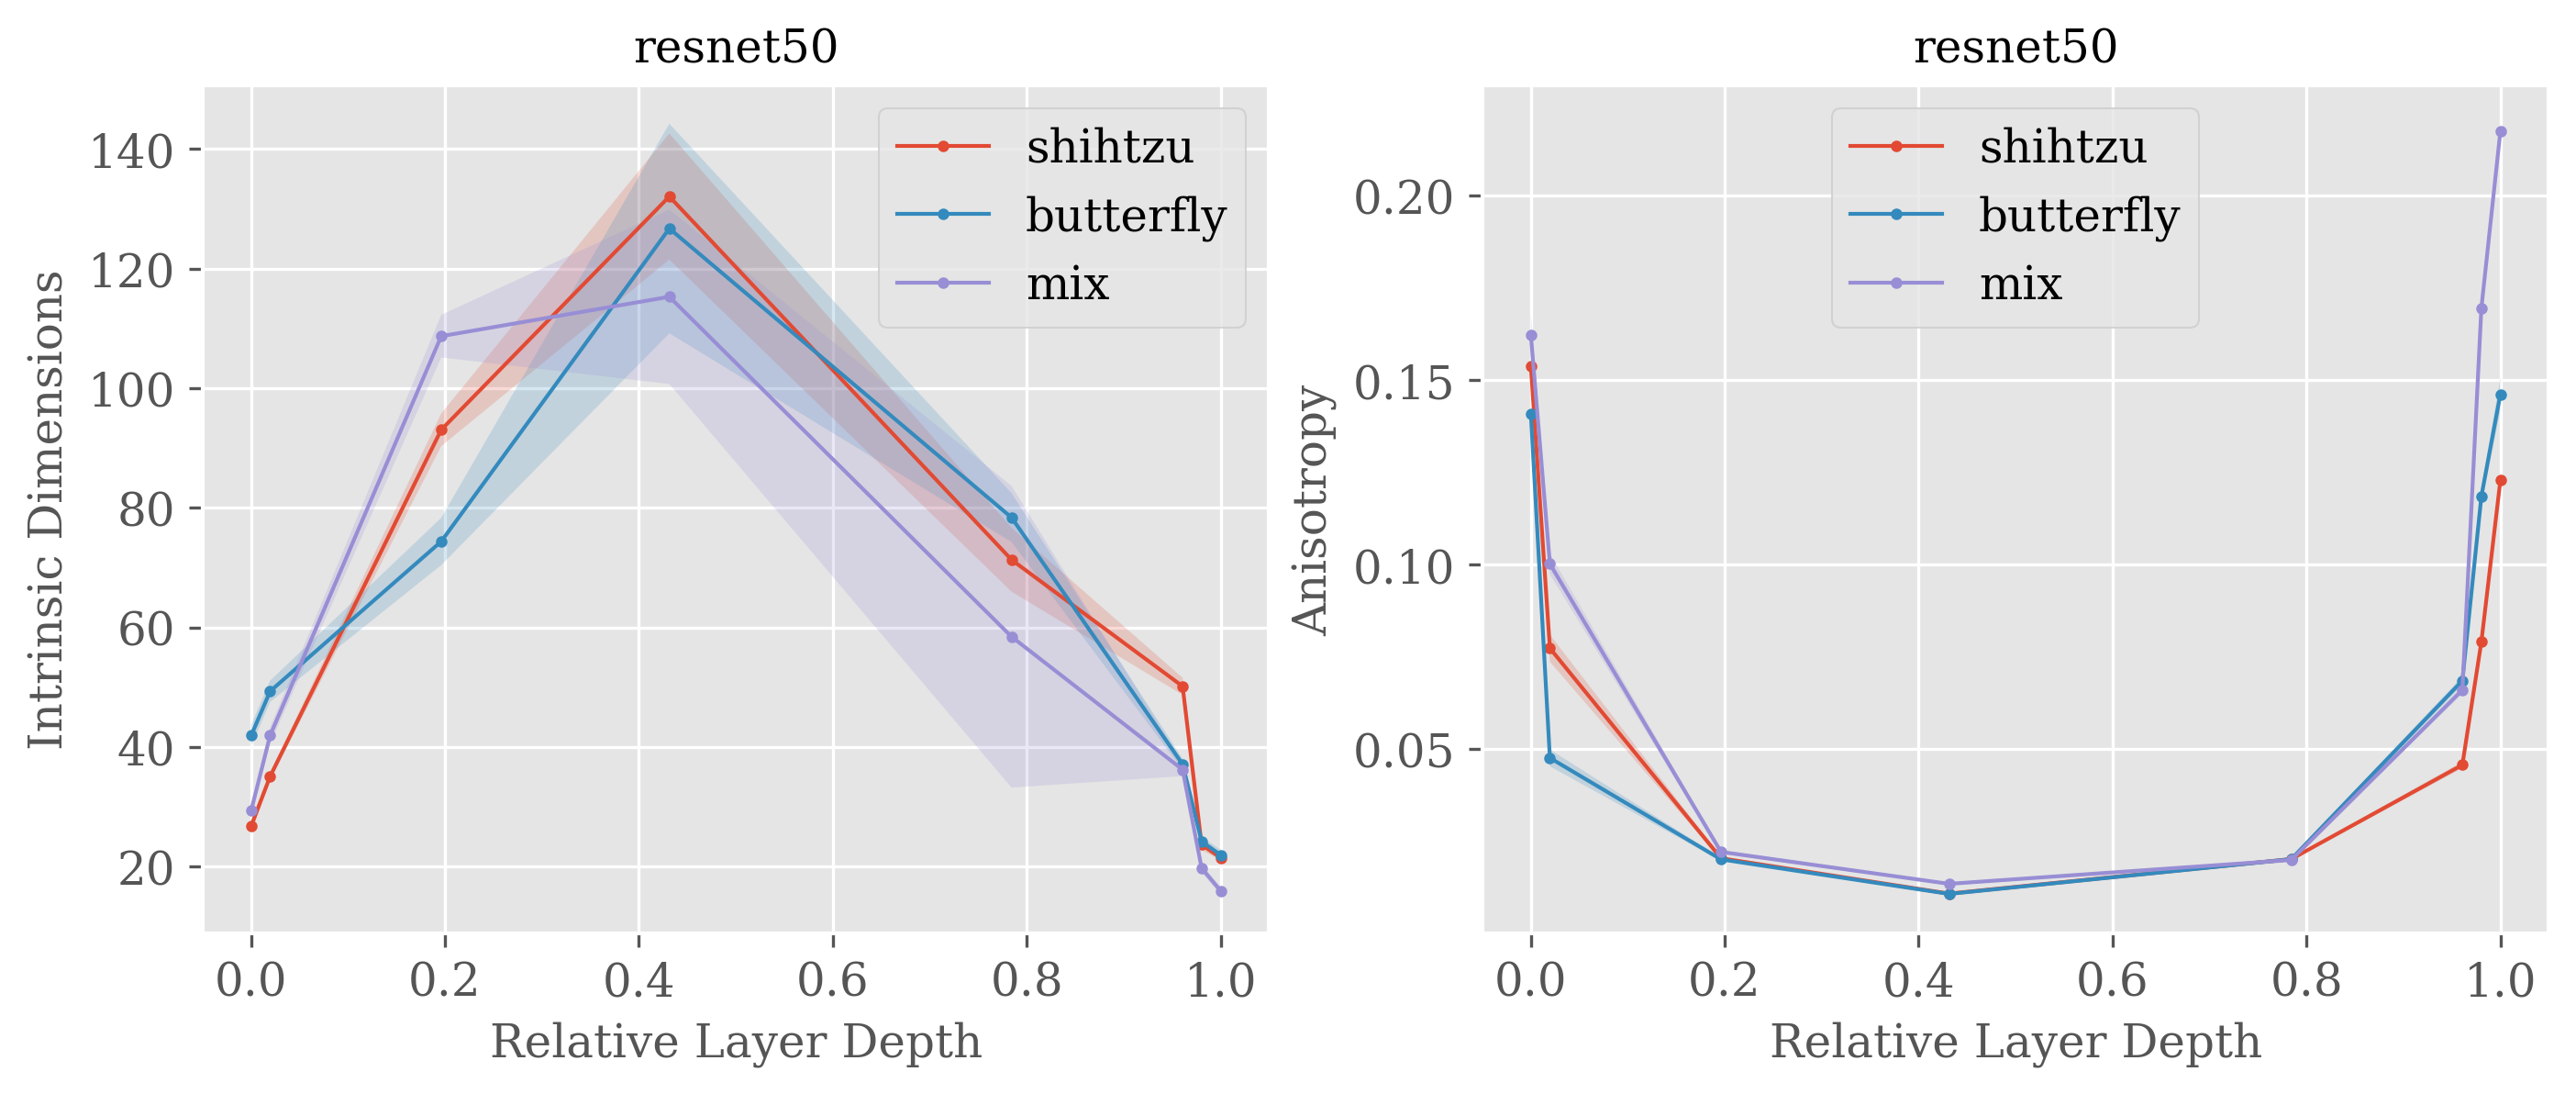
\includegraphics[width=0.75\textwidth]{figures/resnet50_topology.png}
\end{figure}

Then the plots for the vision transformers:
\begin{figure}[h!]
\centering
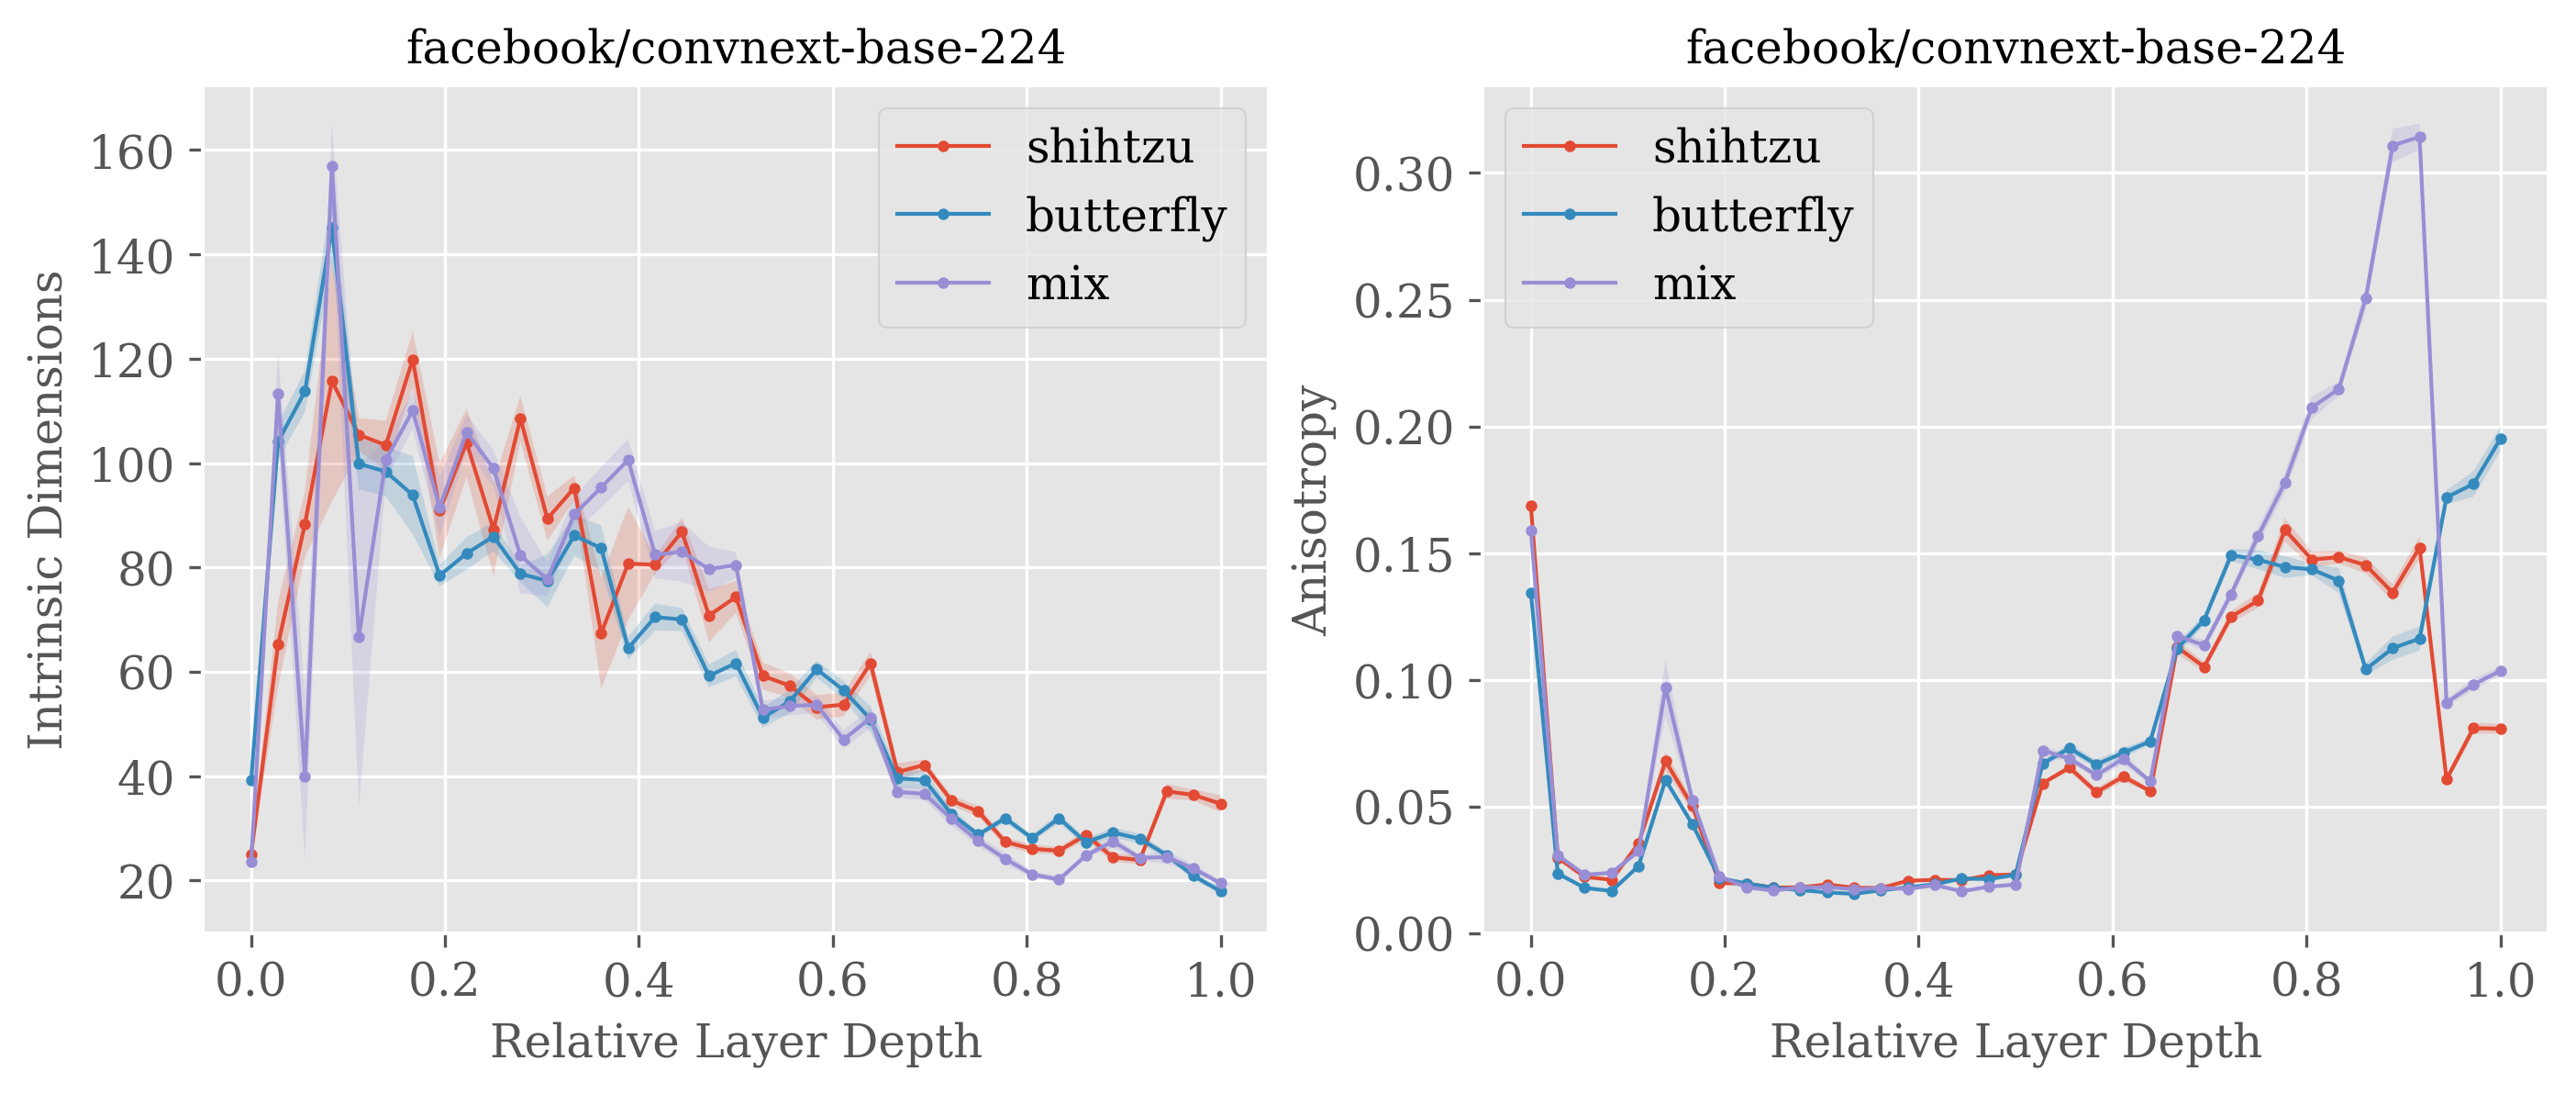
\includegraphics[width=0.75\textwidth]{figures/facebook-convnext-base-224_topology.png}
\end{figure}

\begin{figure}[h!]
\centering
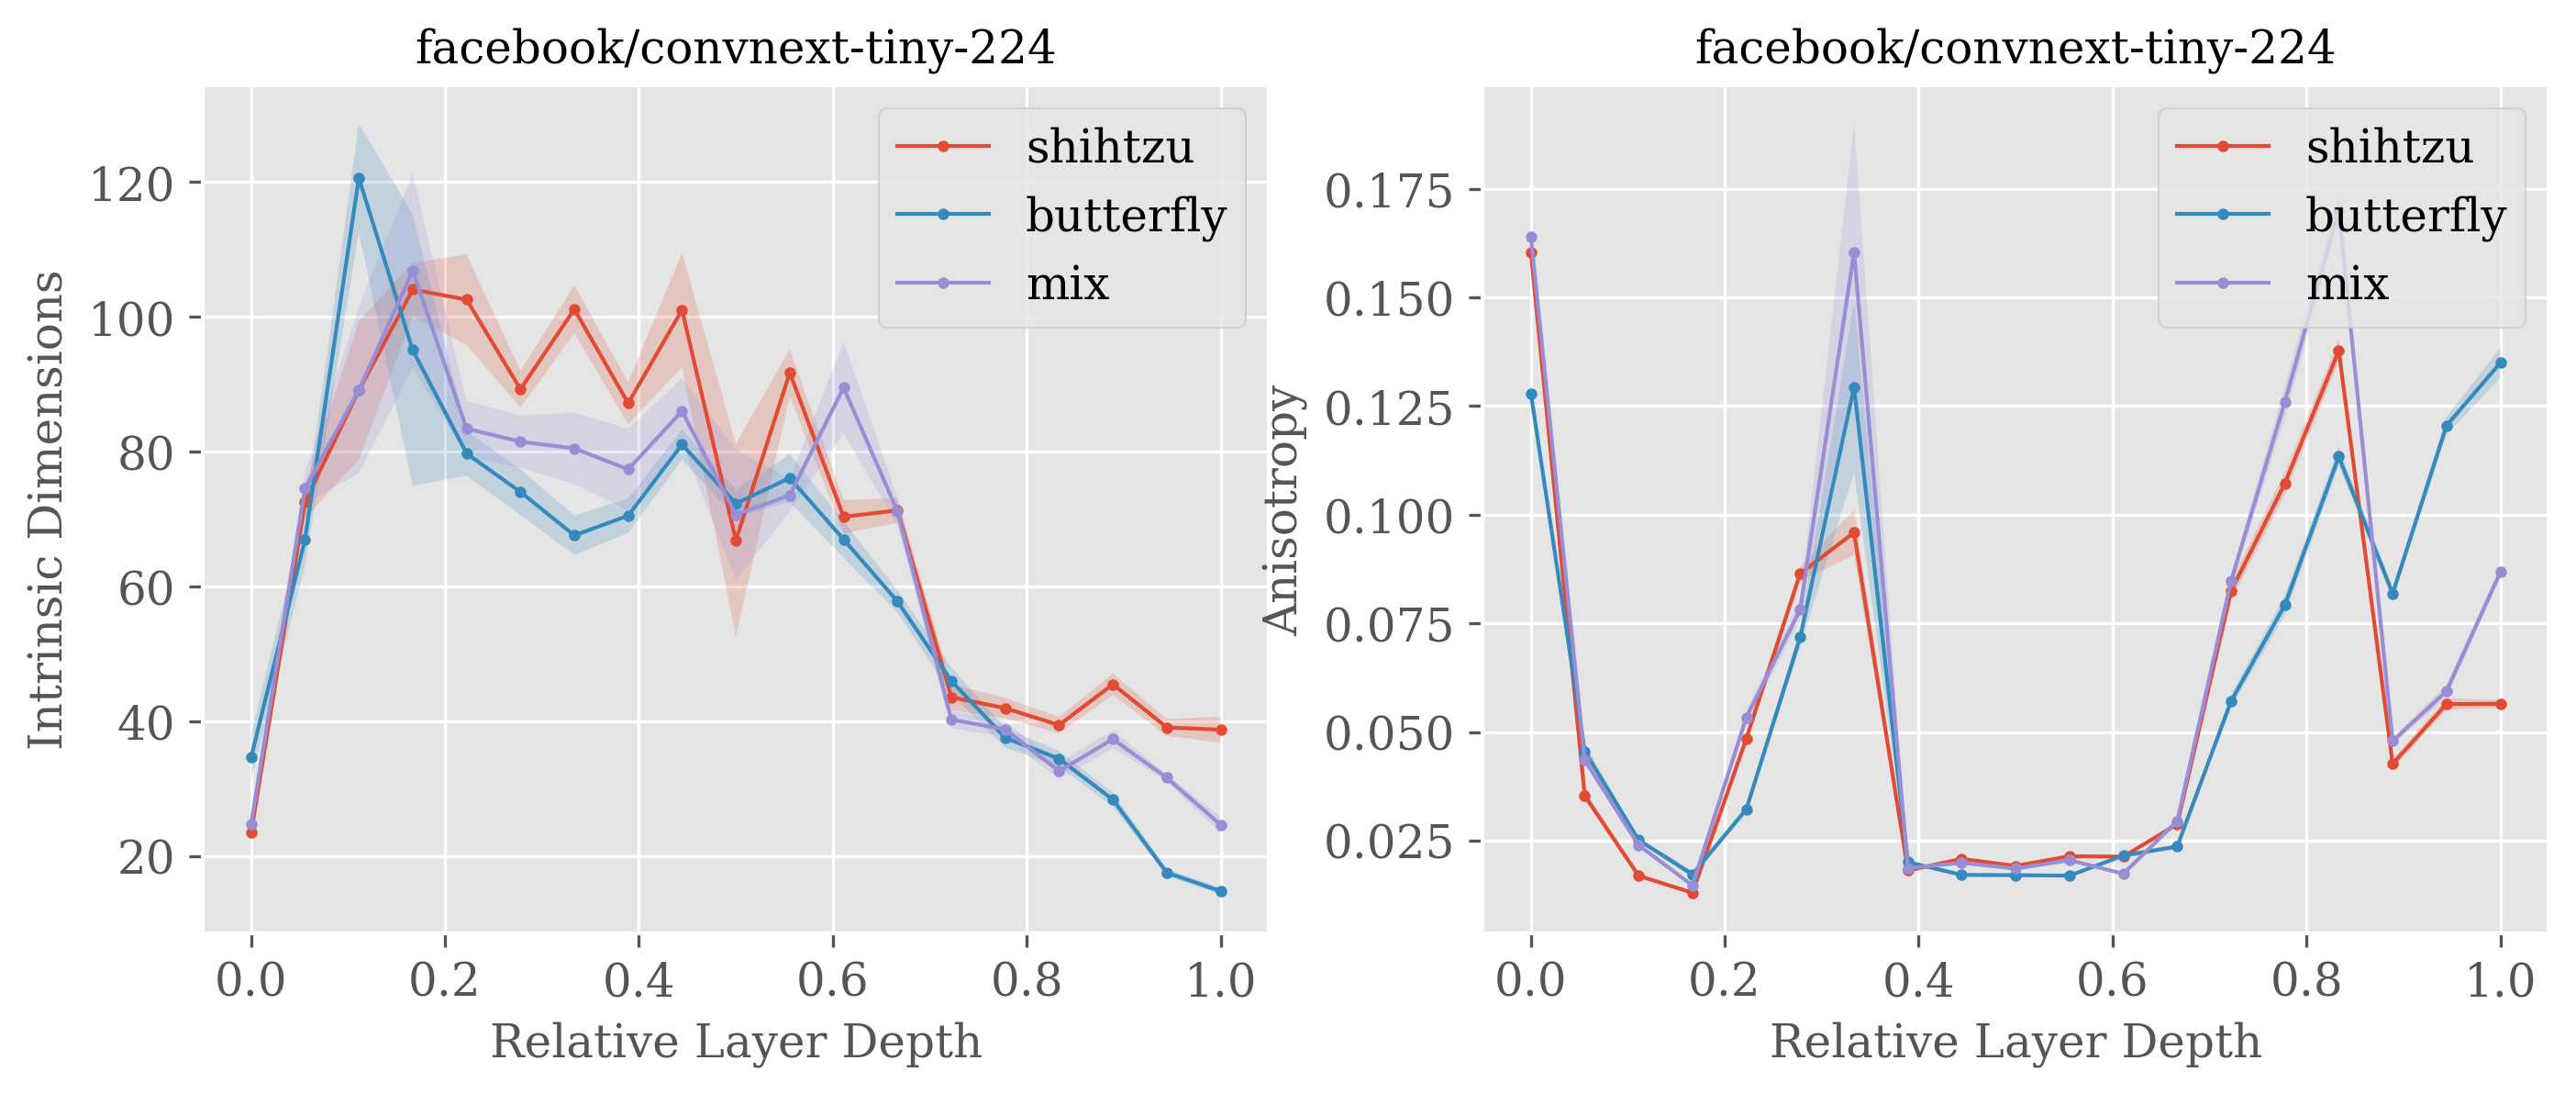
\includegraphics[width=0.75\textwidth]{figures/facebook-convnext-tiny-224_topology.png}
\end{figure}

\begin{figure}[h!]
\centering
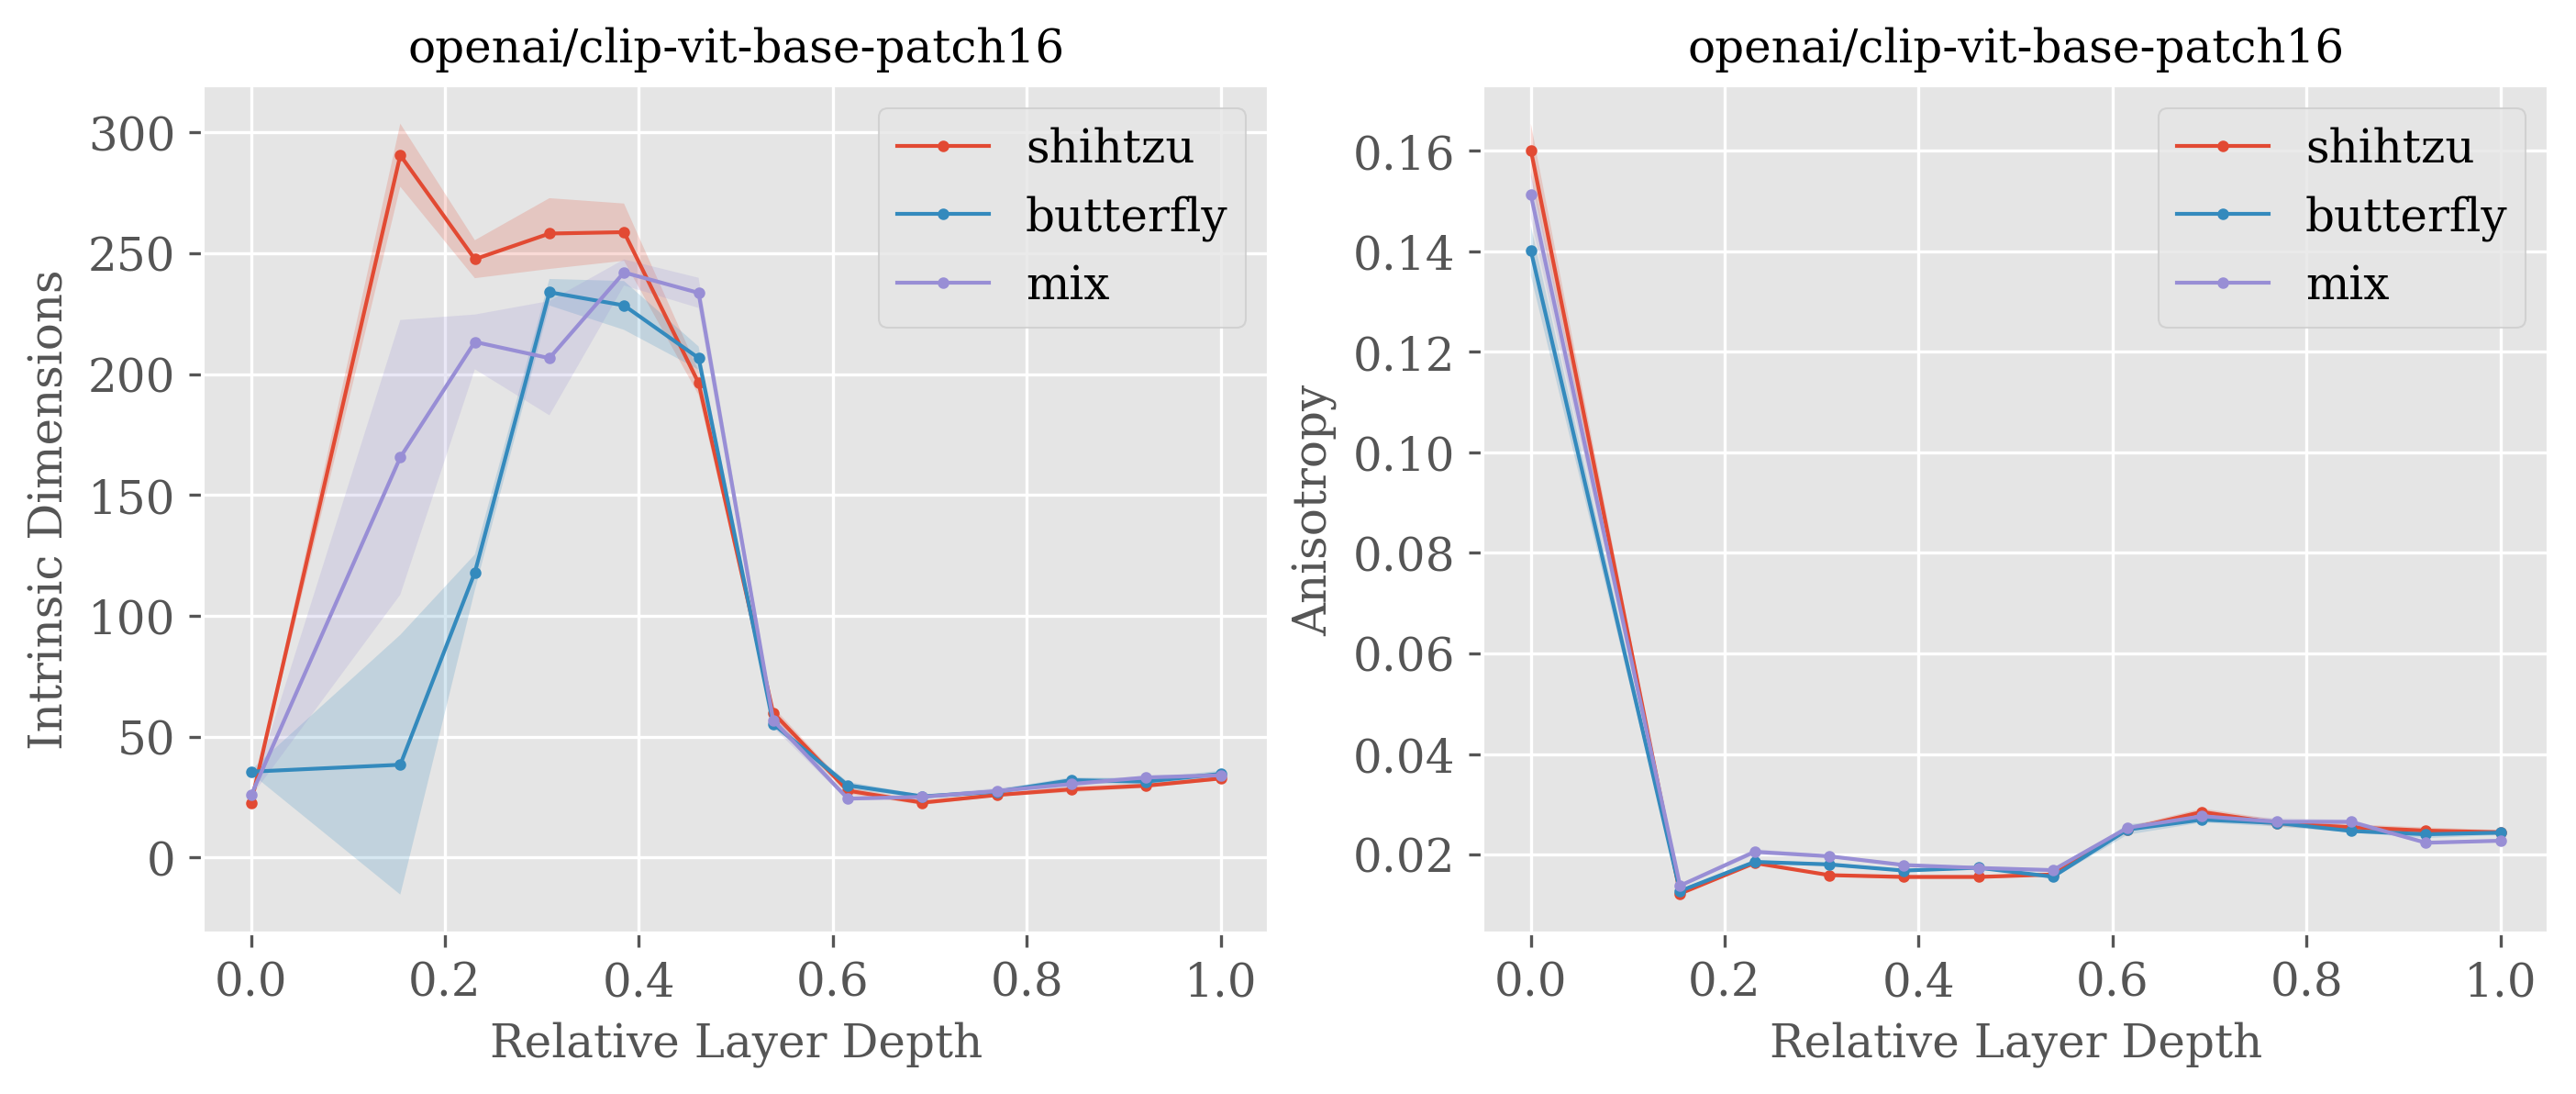
\includegraphics[width=0.75\textwidth]{figures/openai-clip-vit-base-patch16_topology.png}
\end{figure}

\begin{figure}[h!]
\centering
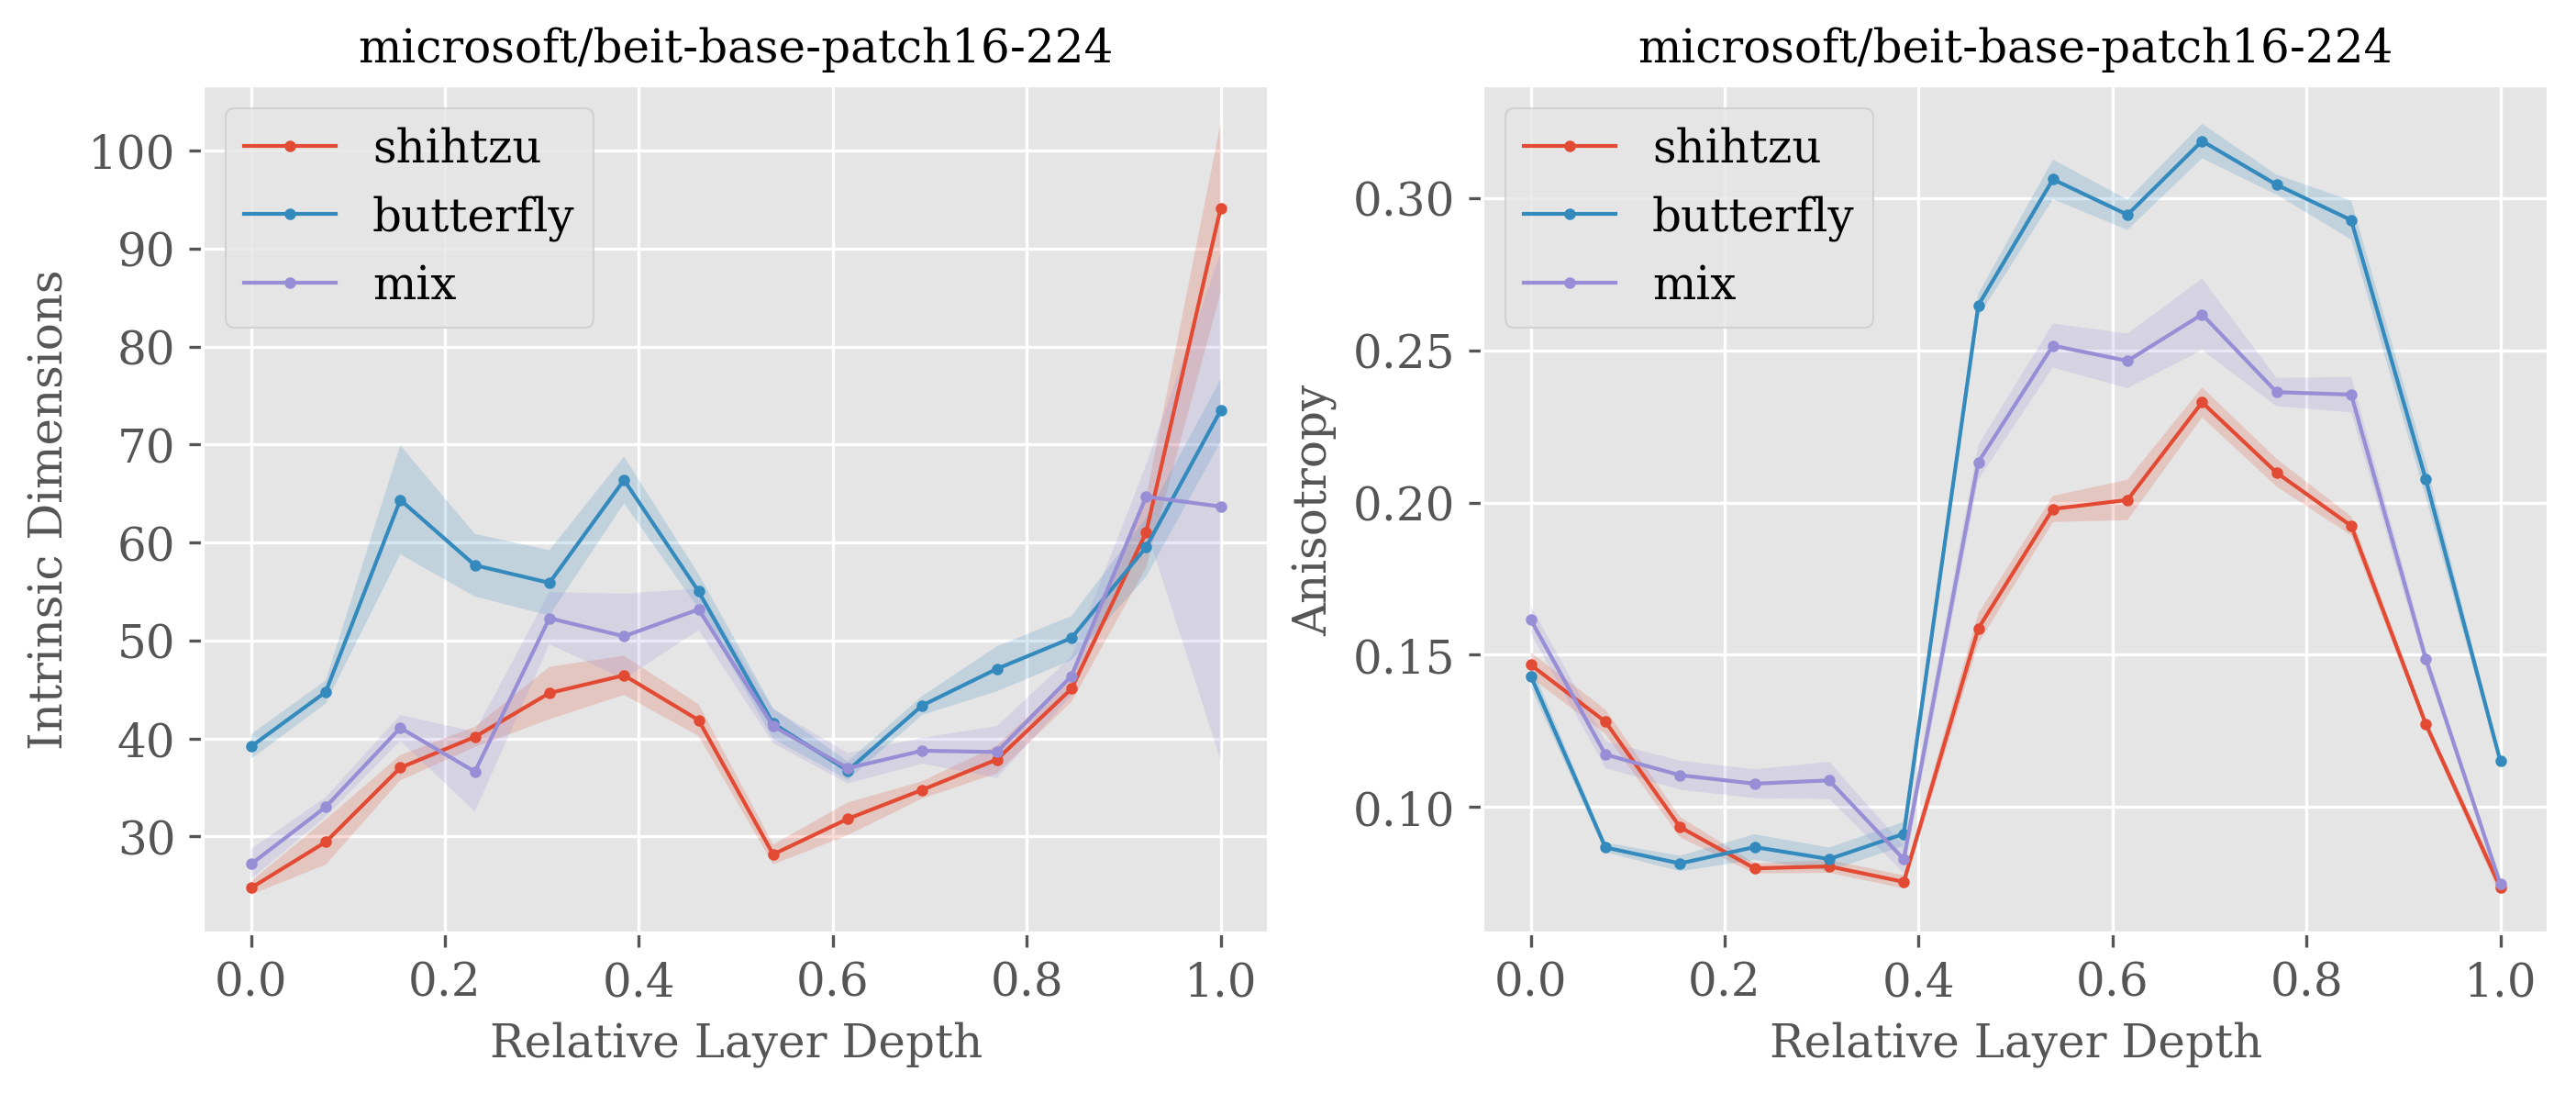
\includegraphics[width=0.75\textwidth]{figures/microsoft-beit-base-patch16-224_topology.png}
\end{figure}

\begin{figure}[h!]
\centering
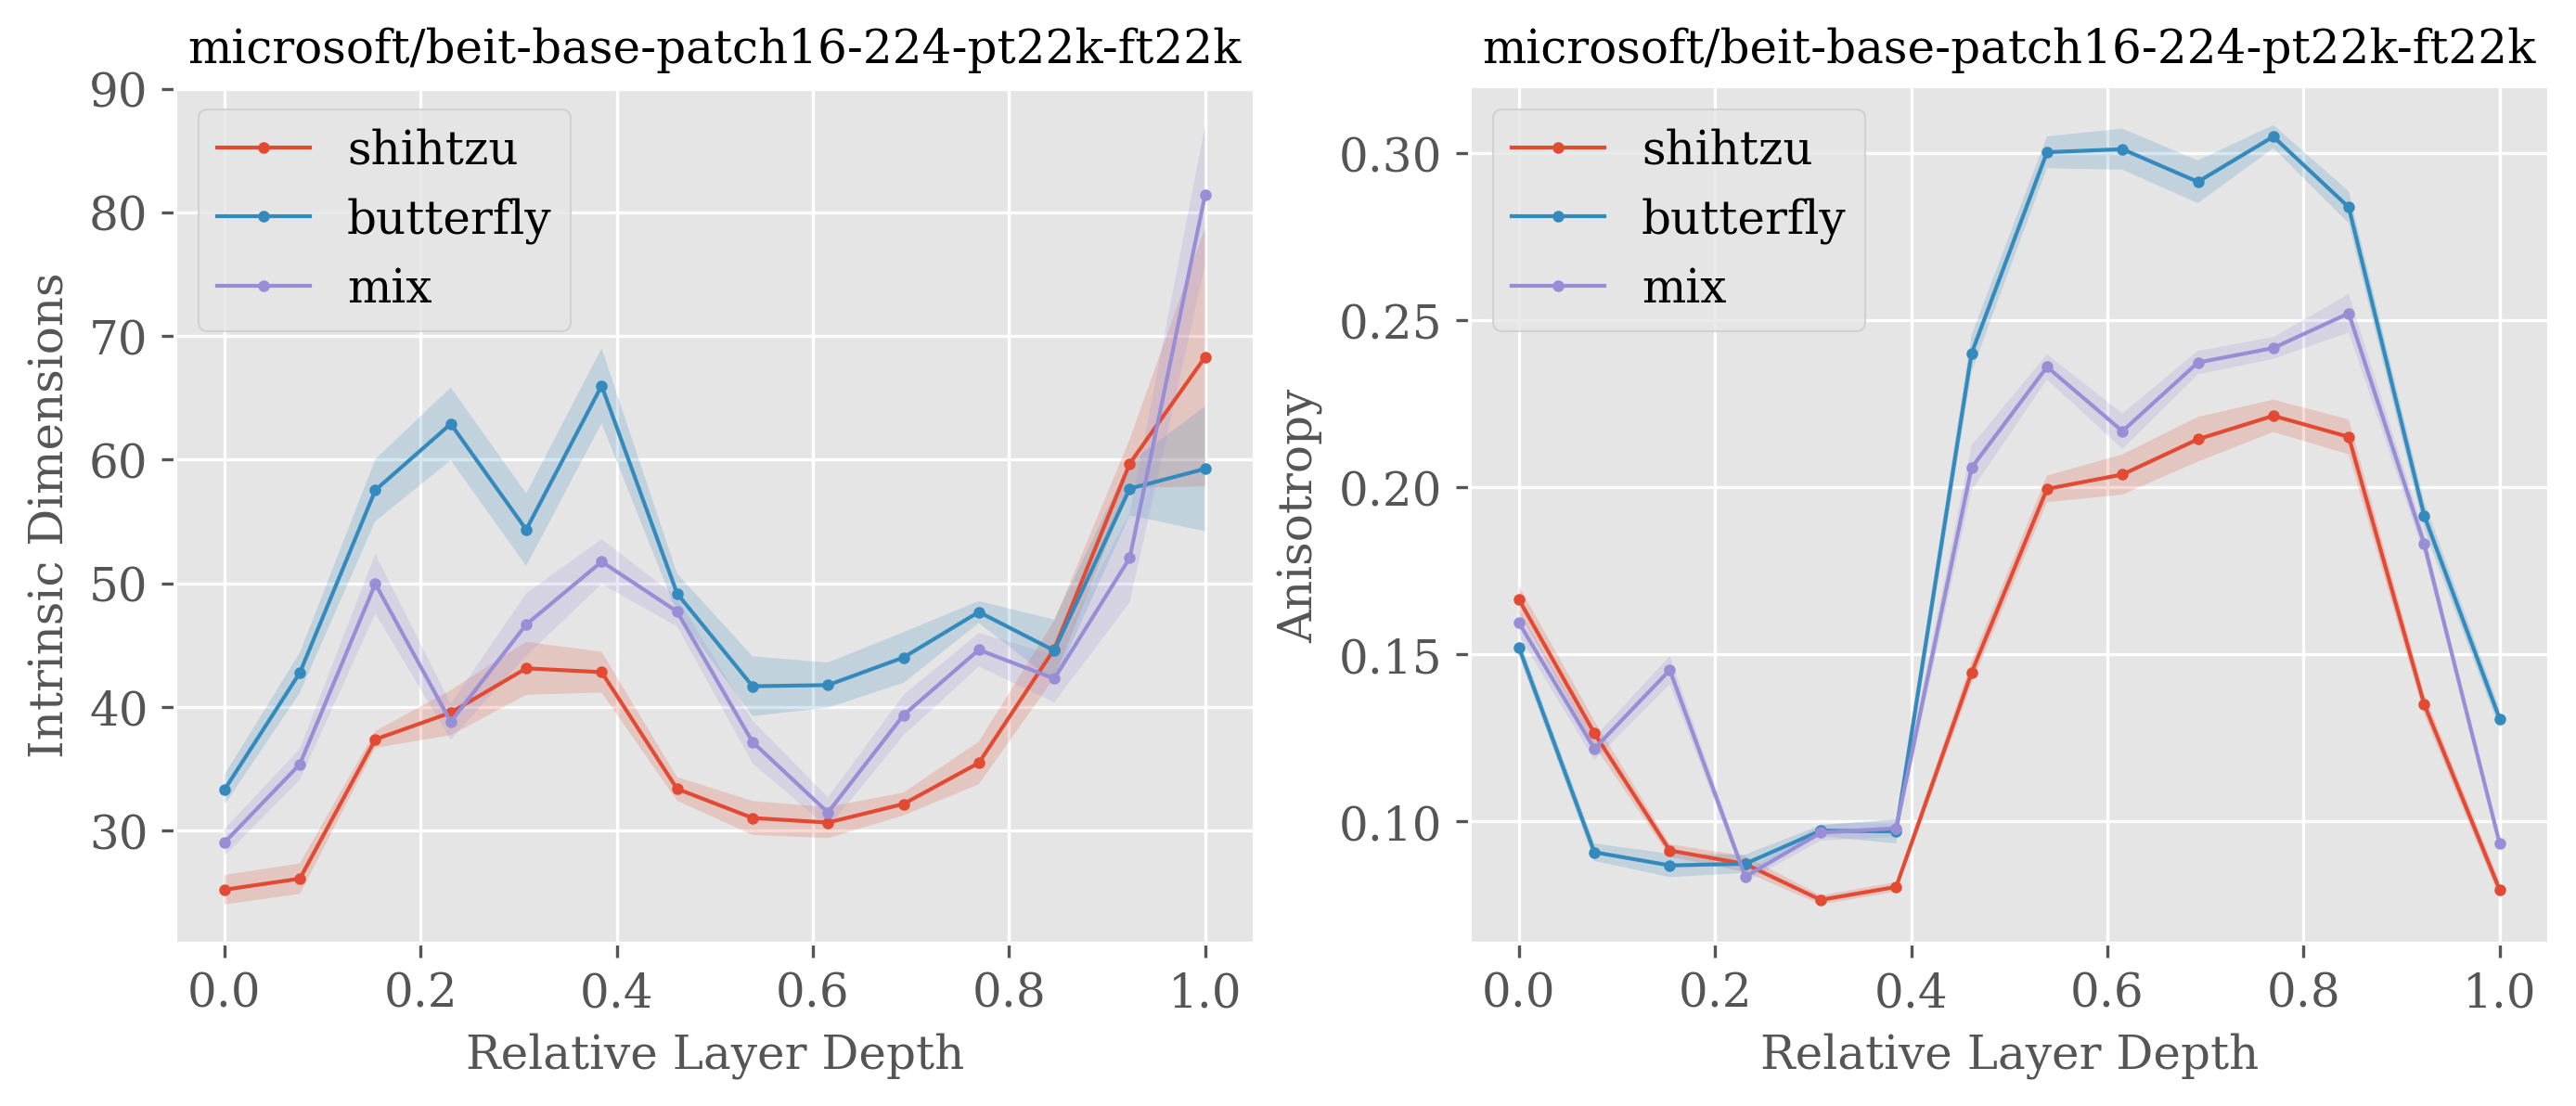
\includegraphics[width=0.75\textwidth]{figures/microsoft-beit-base-patch16-224-pt22k-ft22k_topology.png}
\end{figure}


\section{Internal representations of vision encoder layers (part 2)}\label{part_2}

\subsection{Input embeddings}

For the Vision Transformer (ViT) i.e. the CLIP model \texttt{openai/clip-vit-base-patch16}, the input embedding is computed by first resizing input to a fixed size of $224 \times 224$ pixels and normalizing resulting in a tensor of shape $(BS, 3, 224, 224)$. The images are then split into $16 \times 16$ patches, resulting in $196$ patches for each image. These flattened patches are passed through a linear projection layer to create embeddings of shape $(N, 196, 768)$. Positional encodings of shape $(1, 196, 768)$ are added to keep spatial information.

For ConvNeXt i.e. the \texttt{convnext-base-224}, the input embeddings are similarly obtained by resizing and normalizing the input images to a tensor shape of $(BS, 3, 224, 224)$. However, instead of dividing to patches, ConvNeXt uses several convolutional layers. The output after the initial convolutional layers returns a feature tensor shaped as $(BS, C, H', W')$ where $C$ is the number of channels, and $H'$ and $W'$ are the spatial dimensions after downsampling. The feature map is then pooled or flattened, typically resulting in a shape of $(BS, C \cdot H' \cdot W')$ for subsequent downstream tasks.

In BEiT, \texttt{microsoft/beit-base-patch16-224} the input images are resized and normalized to the shape $(BS, 3, 224, 224)$. The images are divided into $16 \times 16$ patches, resulting in a shape of $(BS, 196, 16 \times 16 \times 3)$. Each patch then tokenized using a pre-trained tokenizer, converting it into discrete tokens, which are then mapped to embeddings through an embedding layer, producing $(N, 196, 512)$. Positional encodings are added to these token embeddings.


\subsection{Linear probing}
Linear probing allows us to analyze the quality of feature representations learned at different layers of the models. By attaching a linear classifier to the outputs of the layers and evaluating its performance on a specific task (e.g. classification), it is possible determine how well the representations capture the relevant information needed for that task. Higher accuracy indicates that the features extracted at that layer are more informative for the classification task.

We can also identify which layers contribute the most to task performance. This can help in understanding how information is processed within the model. E.g., first layers may capture low-level features, while deeper layers may learn more abstract representations. Analyzing performance across layers can reveal the depth at which features become most discriminative for specific tasks.

\subsection{Results}

\begin{figure}[h!] 
\centering
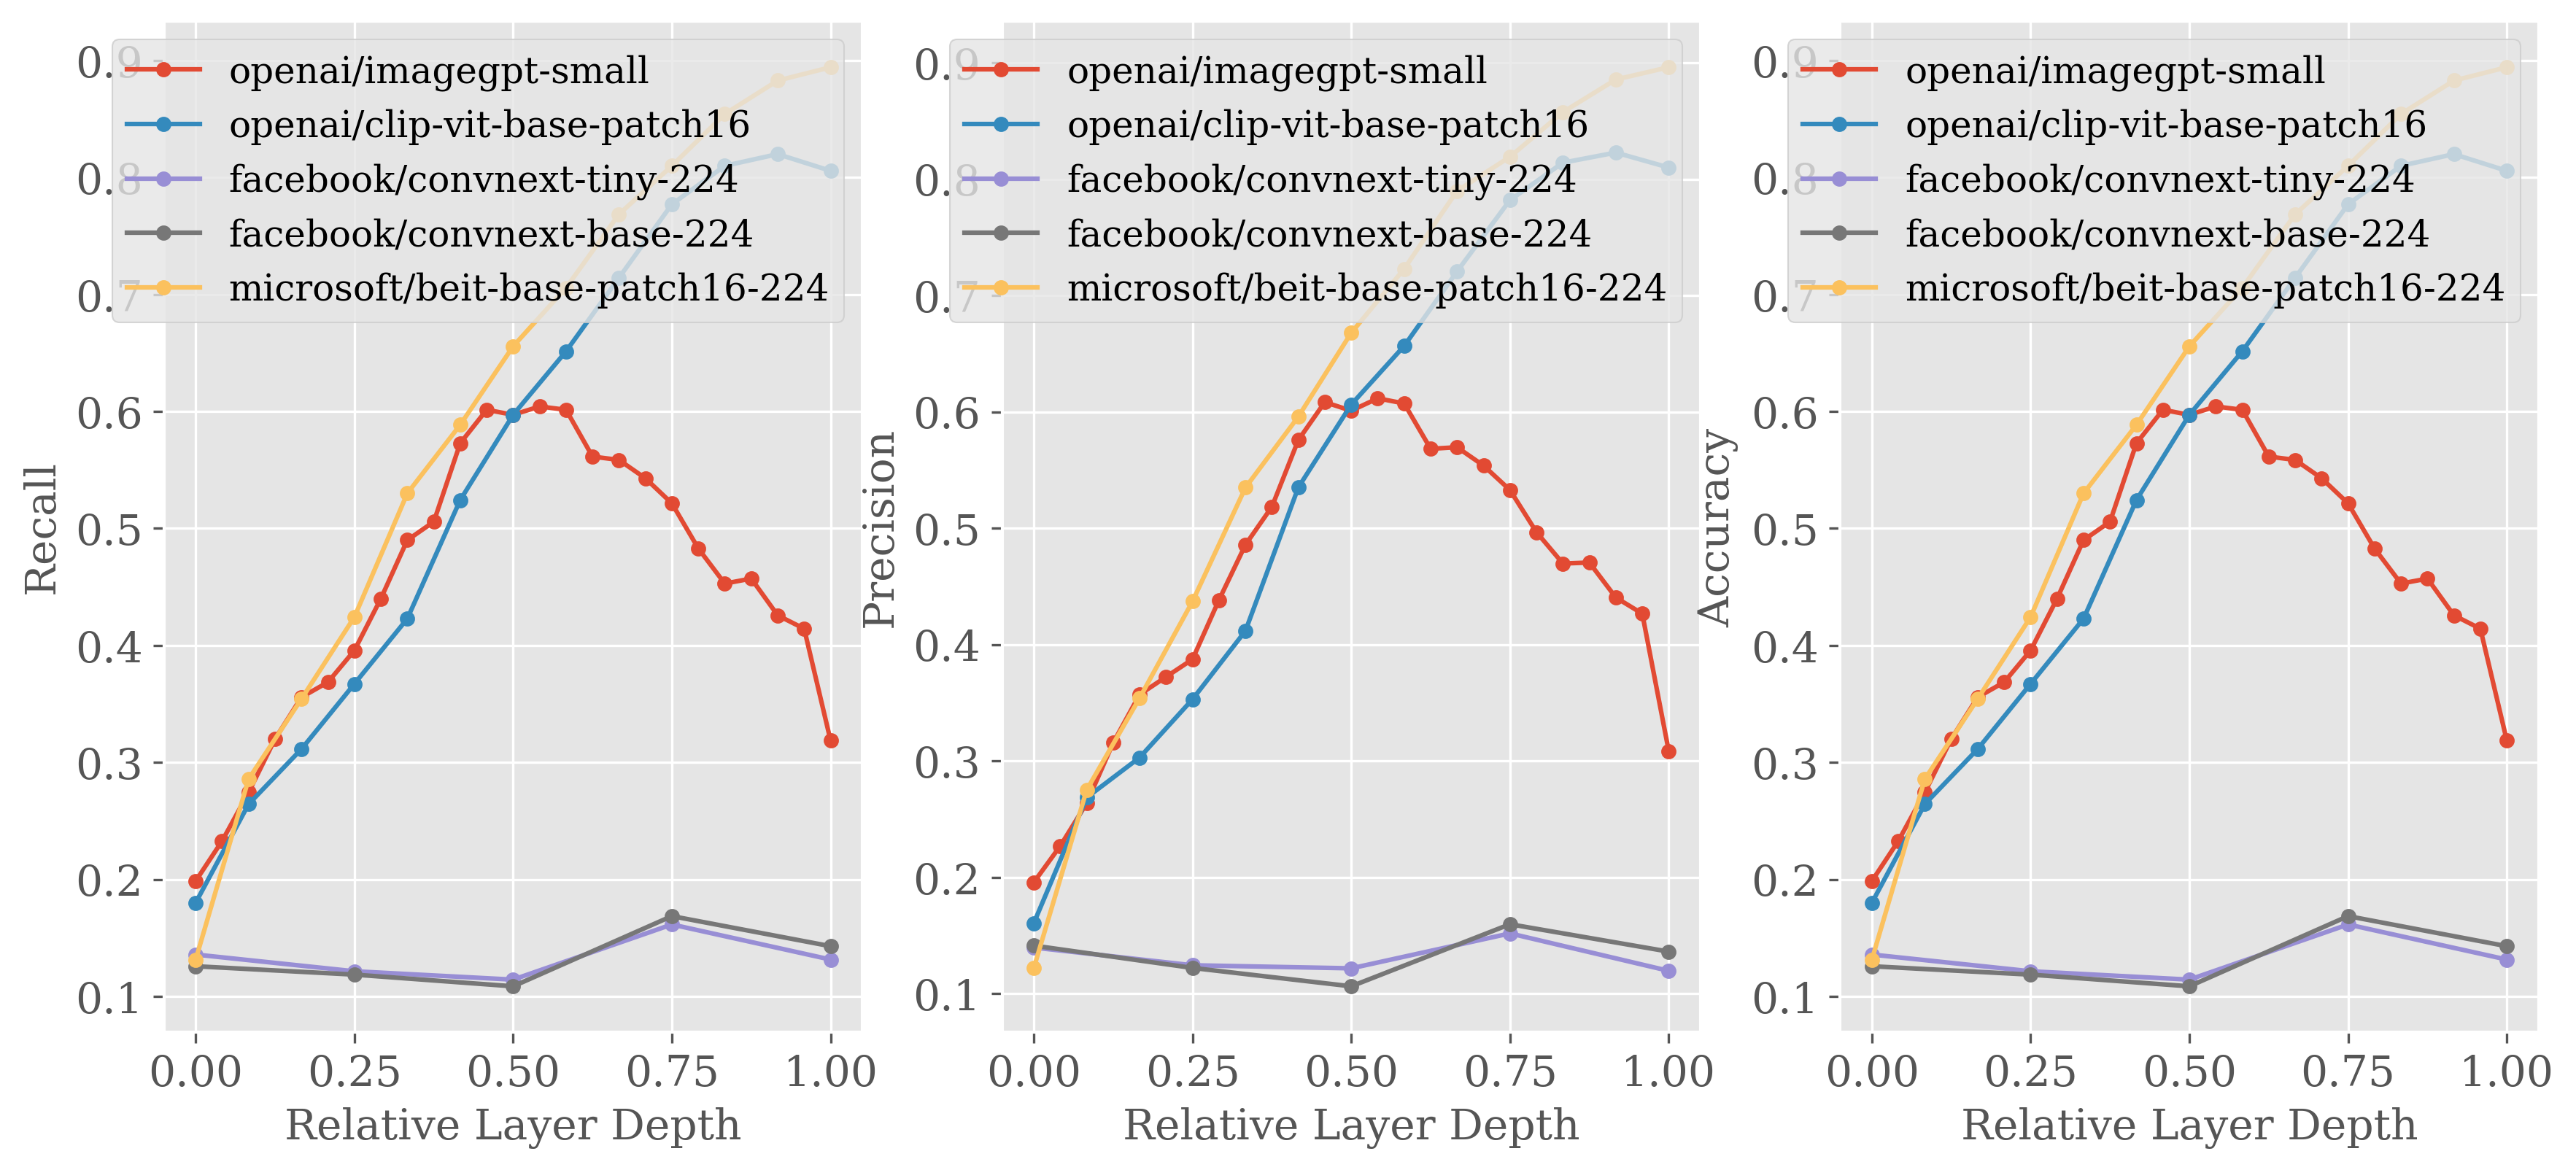
\includegraphics[width=0.85\textwidth]{figures/probing_plots.png}
\end{figure}

As we can see, for the ImageGPT, the best features appear to be obtained in the middle layers, after which performance starts to degrade. In contrast, for ViT-base and BEIT-base, the best features are progressively obtained closer to the output.  

The situation is different for ConvNeXt, where the scores remain consistently low without significant improvement. This could be explained by the flattening operation before classification, which collapses the spatial information (i.e., the 2D structure) into a single vector. This process may result in the loss of valuable spatial relationships within the hidden representations, negatively impacting classifier performance.

\vspace{50pt}
% Bibliography section
\begin{thebibliography}{9}

% Bibliography entry for Facco et al. 2017
\bibitem{facco2017estimating}
Elena Facco, Maria d`Errico, Alex Rodriguez, and Alessandro Laio,
\textit{Estimating the intrinsic dimension of datasets by a minimal neighborhood information},
Scientific Reports, vol. 7, no. 1, pp. 12140, 2017, Nature Publishing Group UK, London.

% Bibliography entry for Ansuini et al. 2019
\bibitem{ansuini2019intrinsic}
  Alessio Ansuini, Alessandro Laio, Jakob H. Macke, and Davide Zoccolan,
  \textit{Intrinsic dimension of data representations in deep neural networks},
  Advances in Neural Information Processing Systems, vol. 32, 2019.

\end{thebibliography}

\end{document}
